\documentclass{standalone}
\usepackage[T1]{fontenc}
\usepackage[utf8]{inputenc}
\usepackage{pgf,tikz}
\usepackage{pgfplots}
\pgfplotsset{compat=1.13}
\usetikzlibrary{shapes}

\begin{document}
\begin{tikzpicture}
  \begin{scope}[xshift=0cm, yshift=0]
    \node[anchor=south west,inner sep=0] (image) at (0,0) {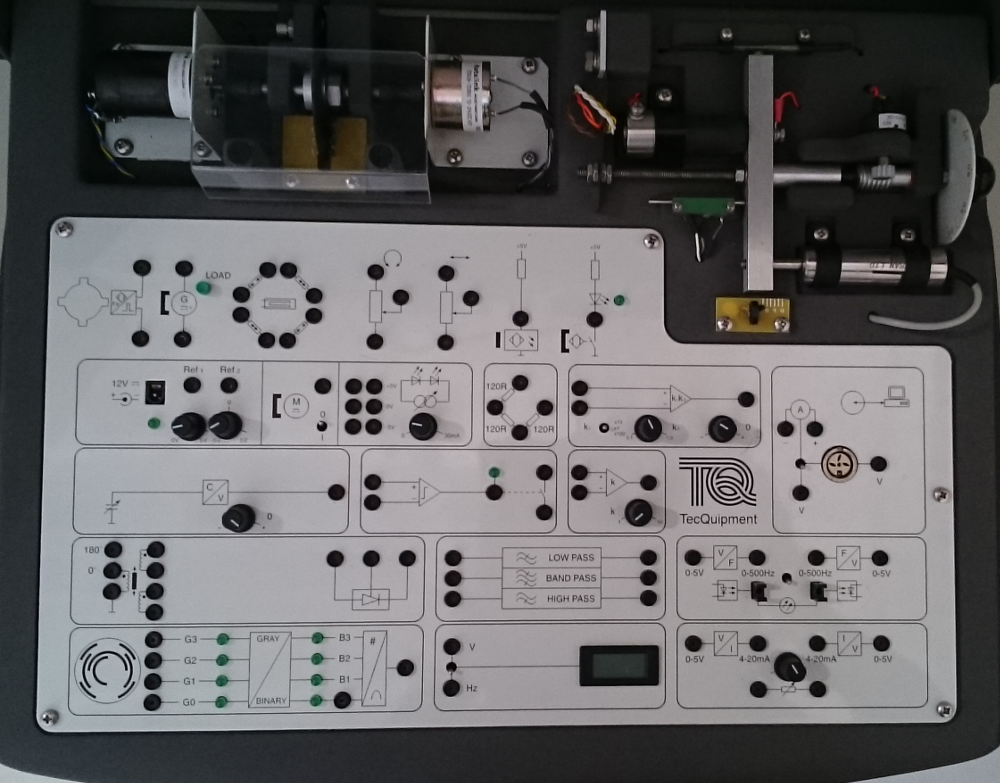
\includegraphics[width=8cm]{TecQbox.png}};
    \begin{scope}[x={(image.south east)},y={(image.north west)}]
        \node[draw, red, rectangle, rounded corners, minimum height=6mm, minimum width=6mm, pin={[pin distance=1mm, color=red] -180:{\scriptsize Voltage source}}] at (0.205, 0.48) {};

        \node[draw, red, rectangle, rounded corners, minimum height=6mm, minimum width=7mm, pin={[pin distance=1mm, color=red] 10:{\scriptsize Motor input and on/off switch}}] at (0.3, 0.48) {};

        \node[draw, red, rectangle, rounded corners, minimum height=8mm, minimum width=4mm, pin={[pin distance=1mm, color=red] 10:{\scriptsize Tachometer output and ground}}] at (0.18, 0.62) {};

        \node[draw, red, rectangle, rounded corners, minimum height=7mm, minimum width=18mm, pin={[pin distance=1mm, color=red] 10:{\scriptsize Voltmeter}}] at (0.55, 0.15) {};

        \node[draw, red, rectangle, rounded corners, minimum height=7mm, minimum width=4mm, pin={[pin distance=1mm, color=red] -180:{\scriptsize Encoder output}}] at (0.405, 0.15) {};

%\draw[help lines,xstep=.1,ystep=.1] (0,0) grid (1,1);
%\foreach \x in {0,1,...,9} { \node [anchor=north] at (\x/10,0) {0.\x}; }
%\foreach \y in {0,1,...,9} { \node [anchor=east] at (0,\y/10) {0.\y}; }
    \end{scope}
  \end{scope}

\end{tikzpicture}
\end{document}
